\ifcsname ifinfulldoc\endcsname\else
    \expandafter\newif\csname ifinfulldoc\endcsname\infulldocfalse
\fi
\ifcsname ifinidedoc\endcsname\else
    \expandafter\newif\csname ifinidedoc\endcsname\inidedoctrue
\fi

\ifinidedoc
\RequirePackage{paralist}
\ifcsname stexdocpath\endcsname\else\def\stexdocpath{.}\fi
\documentclass[full]{l3doc}
%\RequirePackage{document-structure}
\usepackage[hyperref=auto,style=alphabetic]{biblatex}
\usepackage[mathhub=\stexdocpath/mh,usesms]{stex}
\usepackage{stex-highlighting,stexthm}

\newif\ifhadtitle\hadtitlefalse

\def\fileversion{3.3.0}
\def\filedate{\today}
\def\stexdoctitle#1#2{\title{#1\thanks{Version {\fileversion} (last revised {\filedate})} }\def\thispkg{#2}}

\author{Michael Kohlhase, Dennis Müller\\
 	FAU Erlangen-Nürnberg\\
 	\url{http://kwarc.info/}
}

\def\stexmaketitle{\ifhadtitle\else\hadtitletrue\maketitle\fi}

\def\docmodule{
\begin{document}
  \EnableManual
  \DisableImplementation
  \DocInput{\jobname.dtx}
  \EnableImplementation
  \DisableDocumentation
  \DisableManual
  \DocInputAgain
  \clearpage
  \PrintIndex
\end{document}
}

\ExplSyntaxOn
  \bool_new:N \g_stexdoc_typeset_manual_bool
  \NewDocumentCommand \EnableManual {}{
    \bool_gset_true:N \g_stexdoc_typeset_manual_bool
  }
  \NewDocumentCommand \DisableManual {}{
    \bool_gset_false:N \g_stexdoc_typeset_manual_bool
  }
  \NewDocumentEnvironment {stexmanual} {} {
    \bool_if:NTF \g_stexdoc_typeset_manual_bool
      {\bool_set_false:N \l__codedoc_in_implementation_bool}
      {\comment}
  }{
    \bool_if:NF \g_stexdoc_typeset_manual_bool {\endcomment}
  }
\ExplSyntaxOff

%\usepackage{makeidx}
%\makeindex

%\usepackage{document-structure}
\ExplSyntaxOn
\int_new:N \l_stex_docheader_sect

\cs_new_protected:Nn \stexdoc_do_section:n {
  \int_case:nnF \l_stex_docheader_sect {
    {0}{\cs_if_exist:NTF \part {\part{#1}}{
      \int_incr:N \l_stex_docheader_sect
      \stexdoc_do_section:
    }}
    {1}{\cs_if_exist:NTF \chapter {\chapter{#1}}{
      \int_incr:N \l_stex_docheader_sect
      \stexdoc_do_section:
    }}
    {2}{\section{#1}}
    {3}{\subsection{#1}}
    {4}{\subsubsection{#1}}
  }{\paragraph{#1}}
  \int_incr:N \l_stex_docheader_sect
}
%\int_incr:N \l_stex_docheader_sect
\NewDocumentEnvironment{sfragment}{m}{
  \stexdoc_do_section:n{#1}
}{}

\cs_set_nopar:Nn \_stexdoc_do_cs:Nn {
  \stex_debug:nn{here}{\tl_to_str:n{#1},~#2}
  \cs_if_exist:cTF{s\tl_to_str:n{#2}}{
    \cs_if_exist:cTF{s\tl_to_str:n{#2}name}{
    \symref{#2-sym}{#1{#2}}
    }{#1{#2}}
  }{
    #1{#2}
  }
}
\let\my_old_cs\cs
\protected\def\cs#1{
  \_stexdoc_do_cs:Nn \my_old_cs{#1}
}
\let\my_old_cmd\cmd
\protected\def\cmd#1{
  \_stexdoc_do_cs:Nn \my_old_cmd{#1}
}

\ExplSyntaxOff

\mhinput[sTeX/Documentation]{../lib/examples.tex}


\begin{document}

	\title{
		The {\stex} VSCode IDE
		\thanks{Version {\fileversion} (last revised {\filedate})}
 	}
	\author{Michael Kohlhase, Dennis Müller\\
		FAU Erlangen-Nürnberg\\
		\url{http://kwarc.info/}
	}
	\pagenumbering{roman}
	\maketitle

  This is the user manual for the \sTeX Plugin for VSCode, available at
  \url{https://marketplace.visualstudio.com/items?itemName=kwarc.stexide}.
  For the manual for the \sTeX package itself, see \href{\basedocurl/stex-manual.pdf}{the \sTeX{}3 Manual}.
	
	\makeatletter
		\renewcommand\part{%
    		\clearpage
  			\thispagestyle{plain}%
  			\@tempswafalse
  			\null\vfil
  			\secdef\@part\@spart%
  		}
		\newcounter{chapter}
		\numberwithin{section}{chapter}
		\renewcommand\thechapter{\@arabic\c@chapter}
		\renewcommand\thesection{\thechapter.\@arabic\c@section}
		\newcommand*\chaptermark[1]{}
		\setcounter{secnumdepth}{2}
		\newcommand\@chapapp{\chaptername}
		%\newcommand\chaptername{Chapter}
  		\def\ps@headings{%
    		\let\@oddfoot\@empty
    		\def\@oddhead{{\slshape\rightmark}\hfil\thepage}%
    		\let\@mkboth\markboth
    		\def\chaptermark##1{%
      			\markright{\MakeUppercase{%
        			\ifnum \c@secnumdepth >\m@ne
            			\@chapapp\ \thechapter. \ %
        			\fi
        		##1}}%
        	}%
        }
		\newcommand\chapter{\clearpage
			\thispagestyle{plain}%
			\global\@topnum\z@
			\@afterindentfalse
			\secdef\@chapter\@schapter%
		}
		\def\@chapter[#1]#2{\refstepcounter{chapter}%
			\typeout{\@chapapp\space\thechapter.}%
			\addcontentsline{toc}{chapter}%
				{\protect\numberline{\thechapter}#1}%
			\chaptermark{#1}%
			\addtocontents{lof}{\protect\addvspace{10\p@}}%
			\addtocontents{lot}{\protect\addvspace{10\p@}}%
			\@makechapterhead{#2}%
			\@afterheading%
		}
		\def\@makechapterhead#1{%
			\vspace*{50\p@}%
			{\parindent \z@ \raggedright \normalfont
				\huge\bfseries \@chapapp\space \thechapter
				\par\nobreak
				\vskip 20\p@
				\interlinepenalty\@M
				\Huge \bfseries #1\par\nobreak
				\vskip 40\p@
			}%
		}
\newcommand*\l@chapter[2]{%
  \ifnum \c@tocdepth >\m@ne
    \addpenalty{-\@highpenalty}%
    \vskip 1.0em \@plus\p@
    \setlength\@tempdima{1.5em}%
    \begingroup
      \parindent \z@ \rightskip \@pnumwidth
      \parfillskip -\@pnumwidth
      \leavevmode \bfseries
      \advance\leftskip\@tempdima
      \hskip -\leftskip
      #1\nobreak\hfil
      \nobreak\hb@xt@\@pnumwidth{\hss #2%
                                 \kern-\p@\kern\p@}\par
      \penalty\@highpenalty
    \endgroup
  \fi}
\renewcommand*\l@section{\@dottedtocline{1}{1.5em}{2.8em}}
\renewcommand*\l@subsection{\@dottedtocline{2}{3.8em}{3.2em}}
\renewcommand*\l@subsubsection{\@dottedtocline{3}{7.0em}{4.1em}}
\def\partname{Part}
\def\toclevel@part{-1}
\def\maketitle{\chapter{\@title}}
\let\thanks\@gobble
\let\DelayPrintIndex\PrintIndex
\let\PrintIndex\@empty
\providecommand*{\hexnum}[1]{\text{\texttt{\char`\"}#1}}
\makeatother

\ExplSyntaxOn
\int_set:Nn \l_document_structure_section_level_int {1}
\ExplSyntaxOff

\clearpage

{%
  \def\\{:}% fix "newlines" in the ToC
  \tableofcontents
}

\clearpage
\pagenumbering{arabic}

\long\def\ignore#1{}
	
\begin{sfragment}{Setting up the \sTeX Package}

    \begin{sfragment}[id=sec.minimal-setup]{Minimal Setup for the \sTeX Package}
        In the best of all worlds, there is no setup, as you already have a new version of
        {\TeX}Live on your system as a {\LaTeX} enthusiast. If not now is the time to
        install it; see \cite{TeXLive:on}. You can usually update {\TeX}Live via a package
        manager or the {\TeX}Live manager \textbf{tlmgr}.
        \sTeX requires a \TeX{} kernel newer than February 2022. 

        Alternatively, you can install \sTeX from CTAN, the Comprehensive {\TeX} Archive
        Network; see \cite{stexCTAN:on} for details. We
        assume you have the \sTeX package in at least version 3.2 (September 2022).
    \end{sfragment}

    \begin{sfragment}[id=sec.git-setup]{GIT-based Setup for the \sTeX Development Version}
        If you want use the latest and greatest \sTeX packages
        that have not even been released to CTAN, 
        then you can directly clone them from the \sTeX development
        repository \cite{sTeX:github:on} by the following command-line instructions: 
        \begin{lstlisting}[language=bash]
        cd <stexdir>
        git clone https://github.com/slatex/sTeX.git
        \end{lstlisting}
        and keep it updated by pulling updates via \lstinline|git pull| in the cloned \sTeX
        directory.
        Make sure to either clone the \sTeX repository into a local texmf-tree or to update your \lstinline|TEXINPUTS| environment variable, e.g. by placing the following line in your \lstinline|.bashrc|:
        \begin{lstlisting}[language=bash]
        export TEXINPUTS="$(TEXINPUTS):<sTeXDIR>//:"
        \end{lstlisting}       
    \end{sfragment}

      \begin{sfragment}{Setting your MathHub Directory}
    One of \sTeX's features is a proper \emph{module system}
    of interconnected document snippets for mathematical
    content. Analogously to \emph{object-oriented programming},
    it allows for ``object-oriented mathematics'' via individual
    combinable and, importantly, \emph{reusable} modules, developed
    collaboratively.

    To make use of such modules, the \sTeX system needs to be told
    where to find them. There are several ways to do so (see
    \sref[file=stex-mathhub]{sec:localmh}[in=../stex-manual,
        title={\href{\basedocurl/stex-manual.pdf}{the \sTeX{}3 Manual}}]),
    but the most convenient way to do so is via a system variable.

    To do so, create a directory \texttt{MathHub} somewhere on
    your local file system and set the environment
    variable \texttt{MATHHUB} to the file path to that directory.

    In linux, you can do so by writing 
    \begin{lstlisting}[language=bash]
        export MATHHUB="/path/to/your/MathHub"
    \end{lstlisting}
    in your \verb|~/.profile| (for all shells) or \verb|~/.bashrc|
    (for the bash terminal only) file.
  \end{sfragment}
    
\end{sfragment}
\begin{sfragment}{Setting up the \sTeX IDE}
  
    The \sTeX IDE consists of two components using the 
    \emph{Language Server Protocol (LSP)}: A \emph{client}
    in the form of a VSCode extension, and a \emph{server}
    included in the \mmt system. Installing the extension will
    open up a setup routine that will guide you through the rest.
  
    \begin{sfragment}{The \sTeX VSCode Extension}
  
      If you have not already, you should first install the VSCode editor 
      available at \url{https://code.visualstudio.com/}.
  
      Next, open VSCode and install the \sTeX extension by clicking on
      the \emph{extensions} menu on the very left of the VSCode window
      and searching for ``sTeX'' in the 
      \emph{``Search Extensions in Marketplace''} field, as in
      \autoref{fig:install}, and clicking the \emph{Install}-button
      of the \sTeX extension by KWARC.
  
      \begin{figure}
        \begin{center}
          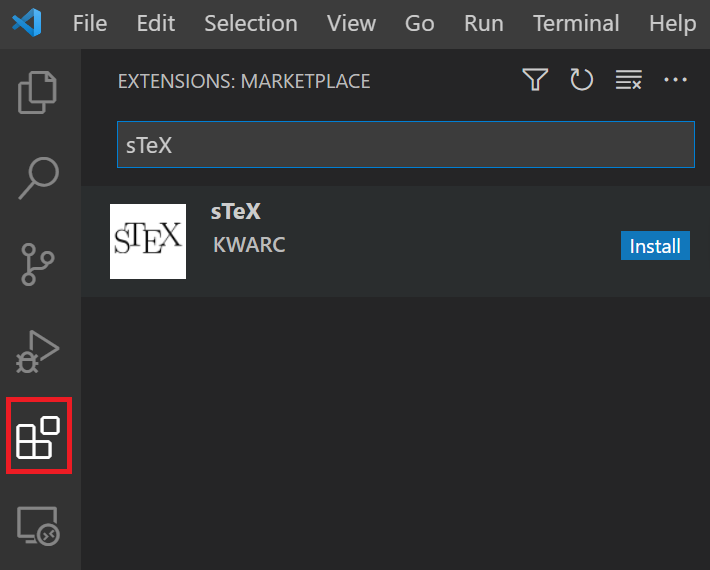
\includegraphics[width=0.6\textwidth]{img/vsc1.png}
        \end{center}
        \caption{Installing the \sTeX extension for VSCode}\label{fig:install}
      \end{figure}
  
    \end{sfragment}
  
    \begin{sfragment}{Setting up \mmt}
  
      Next, open any directory (\texttt{File $\to$ Open Folder...}) that contains
      a \verb|.tex|-file, and a setup window as in \autoref{fig:setup} 
      will pop up. Clik on the highlighted link `\emph{here}' and download
      the latest version of the \texttt{MMT.jar} file (at least version 23.0.0)
      anywhere you like. Then click the \emph{``Browse...''}-button
      and select your freshly downloaded \texttt{MMT.jar}.
  
      If you have already set a system variable for your MathHub-directory,
      you are now done and can click \emph{``Finish''}. If you have not,
      you can now also enter a directory path in the lower text field,
      and the VSCode extension will attempt to globally set one up
      for you, depending on your operating system.
  
      \begin{figure}
        \begin{center}
          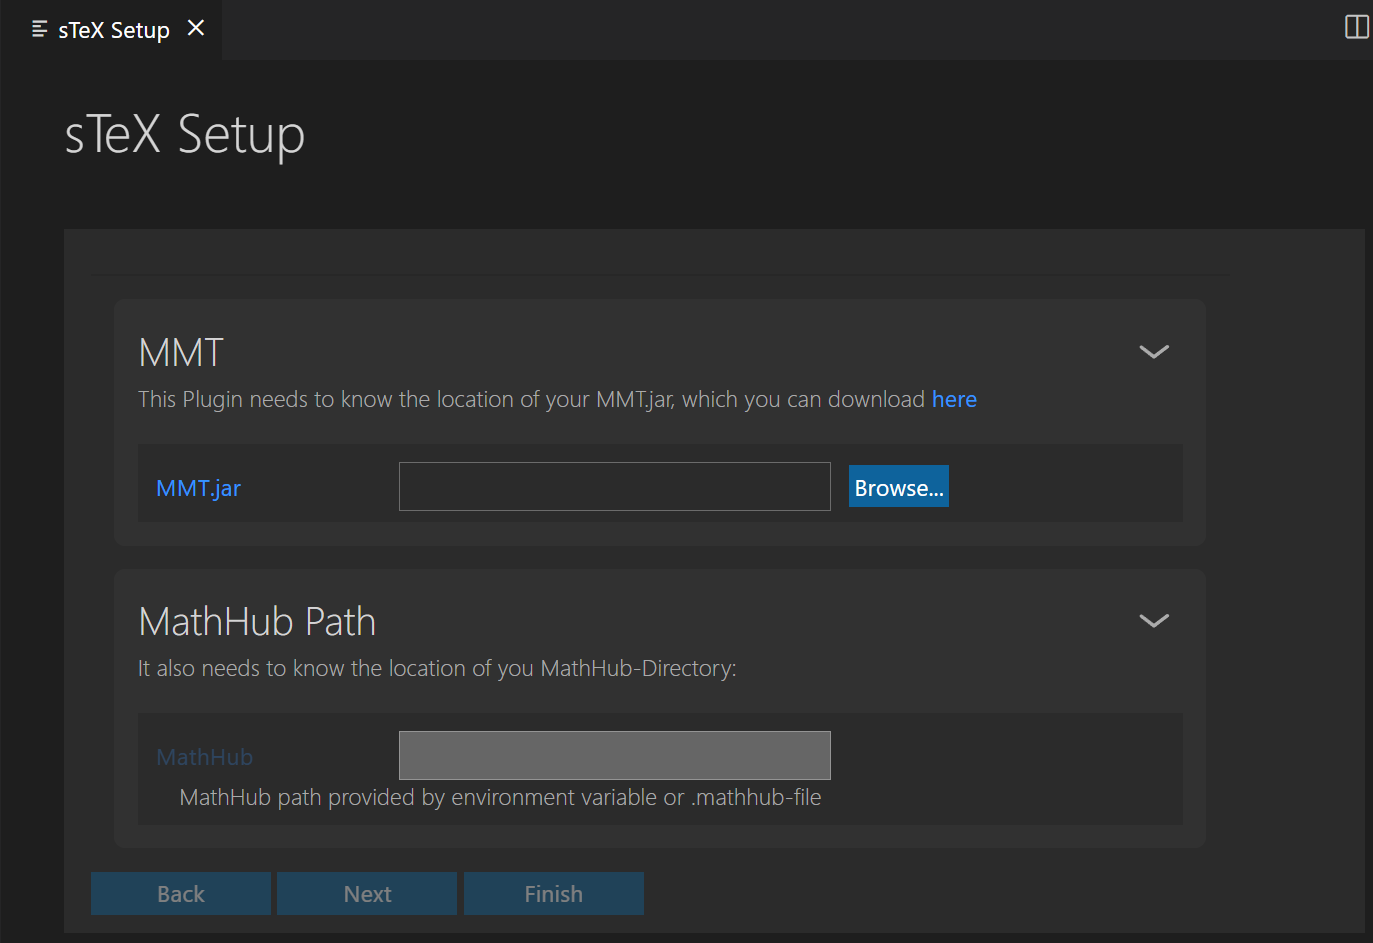
\includegraphics[width=\textwidth]{img/vsc2.png}
        \end{center}
        \caption{\sTeX Setup Routine}\label{fig:setup}
      \end{figure}

      Once you click \emph{``Finish''}, the client will connect
      to \url{https://stexmmt.mathhub.info/:sTeX}, query for
      available archives, download the core libraries required
      for all (or most) semantic services (\texttt{MMT/urtheories}
      and \texttt{sTeX/meta-inf}) and set up \RusTeX for you 
      automatically.
  
    \end{sfragment}
  
  \end{sfragment}

\fi




\ifinidedoc
\newpage 
\printbibliography
\end{document}
\fi


%%% Local Variables:
%%% mode: latex
%%% TeX-master: t
%%% End:

%  LocalWords:  stex-docheader infulldoctrue l@subsubsection toclevel@part ExplSyntaxOff
%  LocalWords:  l_document_structure_section_level_int dangerbox mmtbox omdoc OBJref lmh
%  LocalWords:  own:fifom MueRabRot:rslffml20 sec.stexarchives stex-mathhub ngerman a,b
%  LocalWords:  Metatheory sec.customhighlight sproof stexthm xspace stexpatchmodule
%  LocalWords:  stexpatchexample stexpatchparagraph sexampleid amsthm sassertiontitle
%  LocalWords:  sdefinitiontitle compemph varemph srefsymuri stex-hwexam TeXLive:on tlmgr
%  LocalWords:  stexls:on,stexls-vscode-plugin:on
